%TC:macro \cite [option:text,text]
%TC:macro \citep [option:text,text]
%TC:macro \citet [option:text,text]
%TC:envir table 0 1
%TC:envir table* 0 1
%TC:envir tabular [ignore] word
%TC:envir displaymath 0 word
%TC:envir math 0 word
%TC:envir comment 0 0
%%
%%
%% The first command in your LaTeX source must be the \documentclass command.
\documentclass[acmsmall]{acmart}

\usepackage[utf8]{inputenc}
\usepackage{hyperref}
\usepackage{graphicx}
\usepackage{subcaption}
% \usepackage[margin=1.0in]{geometry}
% \graphicspath{ {./} }
% \usepackage{titlesec}

\usepackage{hyperref}
\hypersetup{
    colorlinks=true, 
    linkcolor=blue, 
    filecolor=magenta,      
    urlcolor=blue,
    }

%% NOTE that a single column version is required for 
%% submission and peer review. This can be done by changing
%% the \doucmentclass[...]{acmart} in this template to 
%% \documentclass[manuscript,screen]{acmart}
%% 
%% To ensure 100% compatibility, please check the white list of
%% approved LaTeX packages to be used with the Master Article Template at
%% https://www.acm.org/publications/taps/whitelist-of-latex-packages 
%% before creating your document. The white list page provides 
%% information on how to submit additional LaTeX packages for 
%% review and adoption.
%% Fonts used in the template cannot be substituted; margin 
%% adjustments are not allowed.
%%
%% \BibTeX command to typeset BibTeX logo in the docs
\AtBeginDocument{%
  \providecommand\BibTeX{{%
    \normalfont B\kern-0.5em{\scshape i\kern-0.25em b}\kern-0.8em\TeX}}}

%% Rights management information.  This information is sent to you
%% when you complete the rights form.  These commands have SAMPLE
%% values in them; it is your responsibility as an author to replace
%% the commands and values with those provided to you when you
%% complete the rights form.
\setcopyright{acmcopyright}
\copyrightyear{2018}
\acmYear{2018}
\acmDOI{XXXXXXX.XXXXXXX}


%%
%% These commands are for a JOURNAL article.
\acmJournal{JACM}
\acmVolume{37}
\acmNumber{4}
\acmArticle{111}
\acmMonth{8}

%%
%% Submission ID.
%% Use this when submitting an article to a sponsored event. You'll
%% receive a unique submission ID from the organizers
%% of the event, and this ID should be used as the parameter to this command.
%%\acmSubmissionID{123-A56-BU3}

%%
%% For managing citations, it is recommended to use bibliography
%% files in BibTeX format.
%%
%% You can then either use BibTeX with the ACM-Reference-Format style,
%% or BibLaTeX with the acmnumeric or acmauthoryear sytles, that include
%% support for advanced citation of software artefact from the
%% biblatex-software package, also separately available on CTAN.
%%
%% Look at the sample-*-biblatex.tex files for templates showcasing
%% the biblatex styles.
%%

%%
%% The majority of ACM publications use numbered citations and
%% references.  The command \citestyle{authoryear} switches to the
%% "author year" style.
%%
%% If you are preparing content for an event
%% sponsored by ACM SIGGRAPH, you must use the "author year" style of
%% citations and references.
%% Uncommenting
%% the next command will enable that style.
%%\citestyle{acmauthoryear}

%%
%% end of the preamble, start of the body of the document source.
\begin{document}

%%
%% The "title" command has an optional parameter,
%% allowing the author to define a "short title" to be used in page headers.
\title{Project Starlink Report}

%%
%% The "author" command and its associated commands are used to define
%% the authors and their affiliations.
%% Of note is the shared affiliation of the first two authors, and the
%% "authornote" and "authornotemark" commands
%% used to denote shared contribution to the research.
\author{Benjamin Kogan}
\authornote{Both authors contributed equally to this research.}
\email{brk57@cornell.edu}
\orcid{1234-5678-9012}
\author{Margia Rounok}
\authornotemark[1]
\email{mr879@cornell.edu}

% \author{Margia Rounok}
% \affiliation{%
%   \institution{The Th{\o}rv{\"a}ld Group}
%   \streetaddress{1 Th{\o}rv{\"a}ld Circle}
%   \city{Hekla}
%   \country{Iceland}}
% \email{larst@affiliation.org}

\author{Robert Zhao}
\affiliation{%
  \institution{Bopha University}
  \city{Guandong}
  \country{China}
}

% \author{Robert Zhao}
% \affiliation{%
%  \institution{Rajiv Gandhi University}
%  \streetaddress{Rono-Hills}
%  \city{Doimukh}
%  \state{Arunachal Pradesh}
%  \country{India}}

% \author{Huifen Chan}
% \affiliation{%
%   \institution{Tsinghua University}
%   \streetaddress{30 Shuangqing Rd}
%   \city{Haidian Qu}
%   \state{Beijing Shi}
%   \country{China}}

% \author{Charles Palmer}
% \affiliation{%
%   \institution{Palmer Research Laboratories}
%   \streetaddress{8600 Datapoint Drive}
%   \city{San Antonio}
%   \state{Texas}
%   \country{USA}
%   \postcode{78229}}
% \email{cpalmer@prl.com}

% \author{John Smith}
% \affiliation{%
%   \institution{The Th{\o}rv{\"a}ld Group}
%   \streetaddress{1 Th{\o}rv{\"a}ld Circle}
%   \city{Hekla}
%   \country{Iceland}}
% \email{jsmith@affiliation.org}

% \author{Julius P. Kumquat}
% \affiliation{%
%   \institution{The Kumquat Consortium}
%   \city{New York}
%   \country{USA}}
% \email{jpkumquat@consortium.net}

%%
%% By default, the full list of authors will be used in the page
%% headers. Often, this list is too long, and will overlap
%% other information printed in the page headers. This command allows
%% the author to define a more concise list
%% of authors' names for this purpose.
\renewcommand{\shortauthors}{Trovato and Tobin, et al.}

%%
%% The abstract is a short summary of the work to be presented in the
%% article.
\begin{abstract}
  A clear and well-documented \LaTeX\ document is presented as an
  article formatted for publication by ACM in a conference proceedings
  or journal publication. Based on the ``acmart'' document class, this
  article presents and explains many of the common variations, as well
  as many of the formatting elements an author may use in the
  preparation of the documentation of their work.
\end{abstract}

%%
%% The code below is generated by the tool at http://dl.acm.org/ccs.cfm.
%% Please copy and paste the code instead of the example below.
%%
\begin{CCSXML}
<ccs2012>
 <concept>
  <concept_id>10010520.10010553.10010562</concept_id>
  <concept_desc>Computer systems organization~Embedded systems</concept_desc>
  <concept_significance>500</concept_significance>
 </concept>
 <concept>
  <concept_id>10010520.10010575.10010755</concept_id>
  <concept_desc>Computer systems organization~Redundancy</concept_desc>
  <concept_significance>300</concept_significance>
 </concept>
 <concept>
  <concept_id>10010520.10010553.10010554</concept_id>
  <concept_desc>Computer systems organization~Robotics</concept_desc>
  <concept_significance>100</concept_significance>
 </concept>
 <concept>
  <concept_id>10003033.10003083.10003095</concept_id>
  <concept_desc>Networks~Network reliability</concept_desc>
  <concept_significance>100</concept_significance>
 </concept>
</ccs2012>
\end{CCSXML}

\ccsdesc[500]{Computer systems organization~Embedded systems}
\ccsdesc[300]{Computer systems organization~Redundancy}
\ccsdesc{Computer systems organization~Robotics}
\ccsdesc[100]{Networks~Network reliability}

%%
%% Keywords. The author(s) should pick words that accurately describe
%% the work being presented. Separate the keywords with commas.
\keywords{datasets, neural networks, gaze detection, text tagging}

\received{20 February 2007}
\received[revised]{12 March 2009}
\received[accepted]{5 June 2009}

%%
%% This command processes the author and affiliation and title
%% information and builds the first part of the formatted document.
\maketitle

\section{Introduction}
Starlink satellites are a network of low Earth orbit satellites designed and operated by SpaceX, a private space exploration company founded by Elon Musk. The aim of Starlink is to provide high-speed, low-latency broadband internet to areas of the world that currently lack reliable internet access. As of April 2023, there are over 1,600 Starlink satellites in orbit, with plans to eventually launch tens of thousands more. The satellites are relatively small and weigh around 260 kg each. They operate in a constellation formation, with each satellite communicating with four others in orbit and with ground stations on Earth.

The Starlink satellites use advanced technology, such as ion thrusters and autonomous collision avoidance systems, to maintain their position in orbit and avoid collisions with other space objects. They are also equipped with advanced lasers to enable communication between satellites and with ground stations, allowing for faster data transfer and lower latency. Moreover, Starlink is a network of low Earth orbit (LEO) satellites designed to provide high-speed, low-latency network connectivity between end hosts on the ground. LEO satellites orbit the Earth at a few hundred kilometers altitude, which allows them to transmit data wirelessly using radio waves between hosts on the ground. This eliminates the need for long-haul fiber connections for transmitting data between hosts in different parts of the world.

The Starlink network has three components: a set of LEO satellites, user terminals, and ground stations. User terminals are purchased and deployed by end-users and wirelessly communicate with the orbiting satellites. Each terminal can only contact a subset of all satellites in orbit, with the satellite map showing which geographical region is within reach of an orbiting satellite. The ground stations act as the other end of the communication and connect user terminals to the fiber infrastructure of the Internet, allowing users to reach the internet infrastructure on the ground.

The project aims to measure latency and network paths between Starlink user terminals and selected Internet destinations over time, capturing variations in latency and comparing profiles of different user terminals.

\section{Methodology}
RIPE Atlas Cousteau is a tool used for conducting measurements on the Internet, such as measuring latency, traceroutes, and DNS queries. The tool is part of the RIPE Atlas project, which is a large-scale, globally distributed network measurement infrastructure operated by the RIPE NCC. To use RIPE Atlas Cousteau for conducting measurements, we first need to register an account with the RIPE NCC and obtain an API key. The API key is required to access the RIPE Atlas API, which allows us to submit measurement requests and retrieve measurement results. Once we have obtained the API key, we can use Python programming language and the Cousteau library to interact with the RIPE Atlas API. We can then write Python scripts that use the Cousteau library to submit measurement requests, retrieve measurement results, and perform data analysis.

To conduct measurements using RIPE Atlas Cousteau, we first need to define the measurement parameters, such as the target IP address, the measurement type (e.g., ping, traceroute), and the measurement interval (whether it’s one-off or in an appropriate start and stop time interval). We can then submit the measurement request to the RIPE Atlas API using the Cousteau library. After the measurement is completed, we can retrieve the measurement results from the RIPE Atlas API using the Cousteau library. We can then analyze the results using Python libraries such as Pandas and Matplotlib to visualize the data and draw conclusions.

Overall, we used the RIPE Atlas Cousteau for conducting Internet measurements which  involved registering an account, obtaining an API key, writing Python scripts using the Cousteau library, submitting measurement requests, retrieving measurement results, and performing data analysis.

\section{Data and Results}
Once we have gotten the proper spawning pings, we make a create measurement request to collect the data over the span of a day. 

\subsection{General}

\begin{figure}
    \centering
    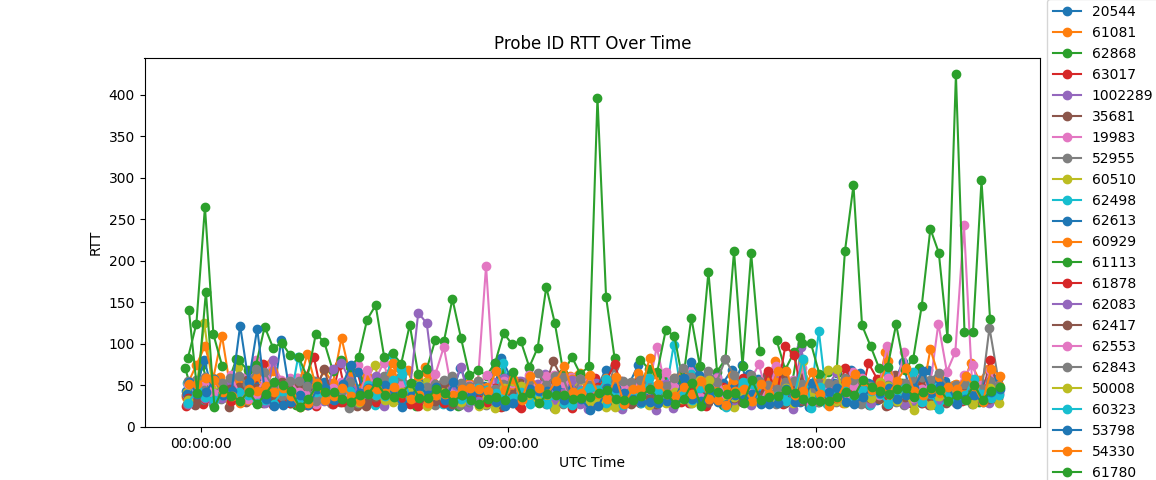
\includegraphics[scale=0.4]{graphs/general.png}
    \caption{Plot of each probe over time}
    \label{fig:general}
\end{figure}%

Our measurement returned 23 international probes from three distinct geographical regions: North America, Europe, and Oceania. The majority of these probes emanated from the United States of America, totaling thirteen in number, followed by Germany with three probes, and Australia with two probes. The remaining probes originated from Poland, the United Kingdom, France, Canada, and Austria, with a solitary representation each. In general, our measurements were a success. All probes were able to respond to the measurement request with the exception of probe ID 61113 (from USA) which was unreachable and had 100 percent packet loss. Interestingly, the remainder of the probes had 0 percent packet loss. Finally, due to the rate-limiting of the RIPE Atlas API (there cannot be more than 25 concurrent requests), we decided to use a number of probe IDs that were close to the threshold but would not too close as it might have impacted the data collection during mid-execution.  

Our analysis of the acquired probes did not reveal any discernible patterns or trends across all probes. However, we did observe periodic and cyclic changes in the Round Trip Time (RTT) metric. Specifically, we detected fluctuations in RTT measurements, where the RTT time experienced peak highs followed by lows in a cyclical manner over the span of a day. This observation suggests that the underlying network infrastructure may be subject to intermittent congestion or routing issues, which can result in fluctuations in the latency of network traffic. Further analysis is required to ascertain the root cause of these RTT variations and their potential impact on network performance. As such, we decided to dig deeper into the regional patterns of latency across the probes. 

\subsection{Regional}
We looked at the locations of our probes and split them geographically to see if there are any trends.

\subsubsection{USA1}
\begin{figure}
    \centering
    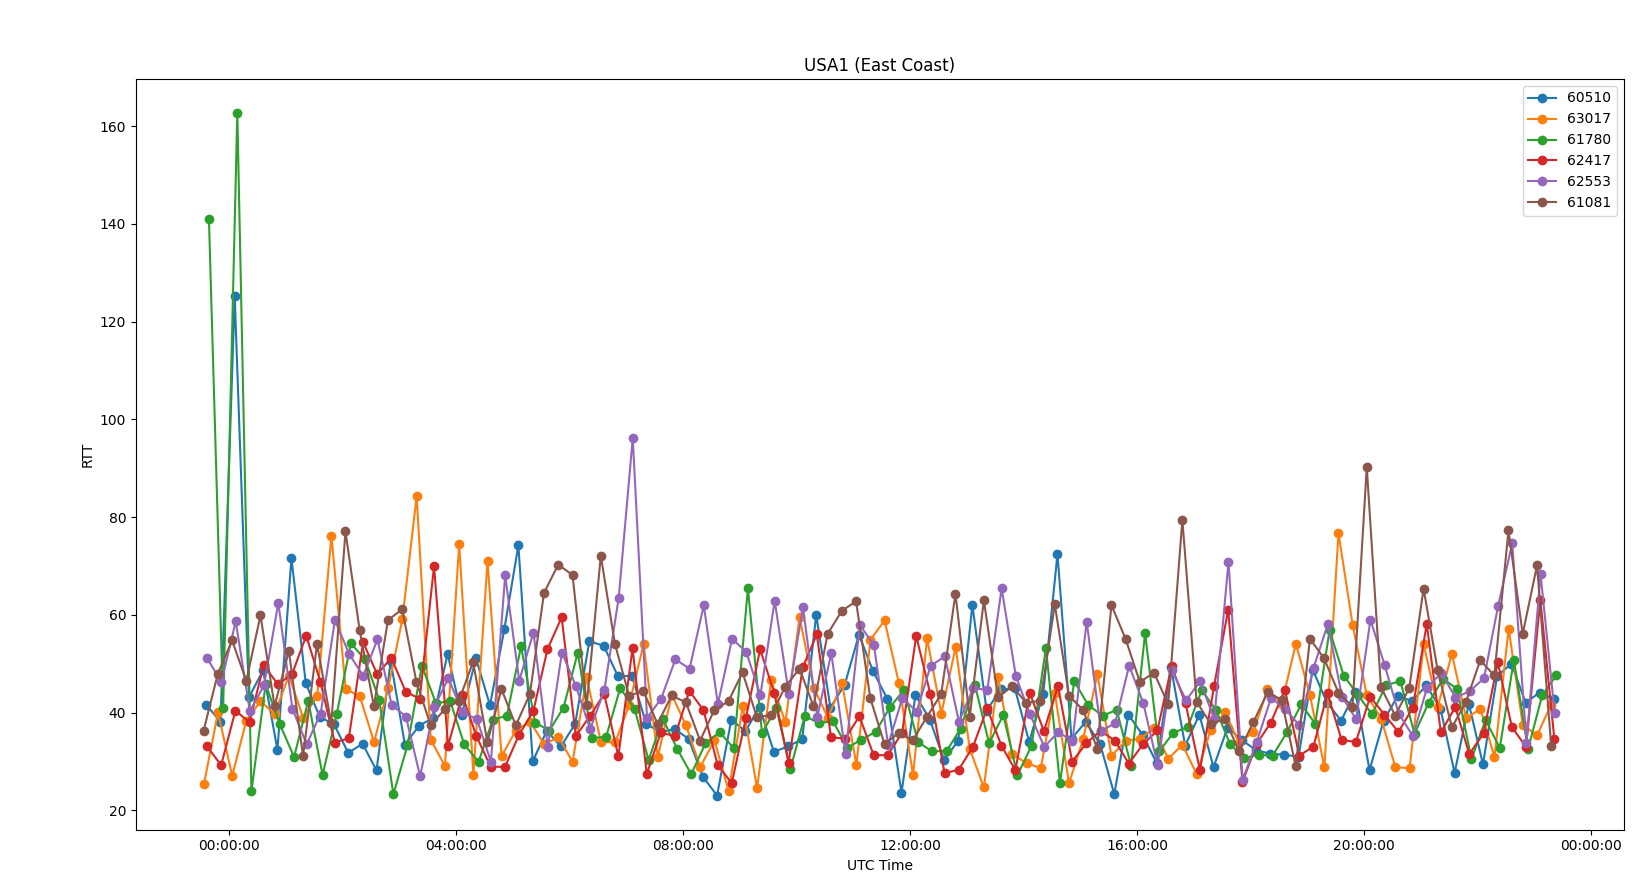
\includegraphics[scale=0.3]{graphs/usa1.png}
    \caption{Graph of RTT vs. UTC Time for the East Coast}
    \label{fig:my_label}
\end{figure}
    
TODO: describe east coast data 

\subsubsection{USA2}
\begin{figure}
    \centering
    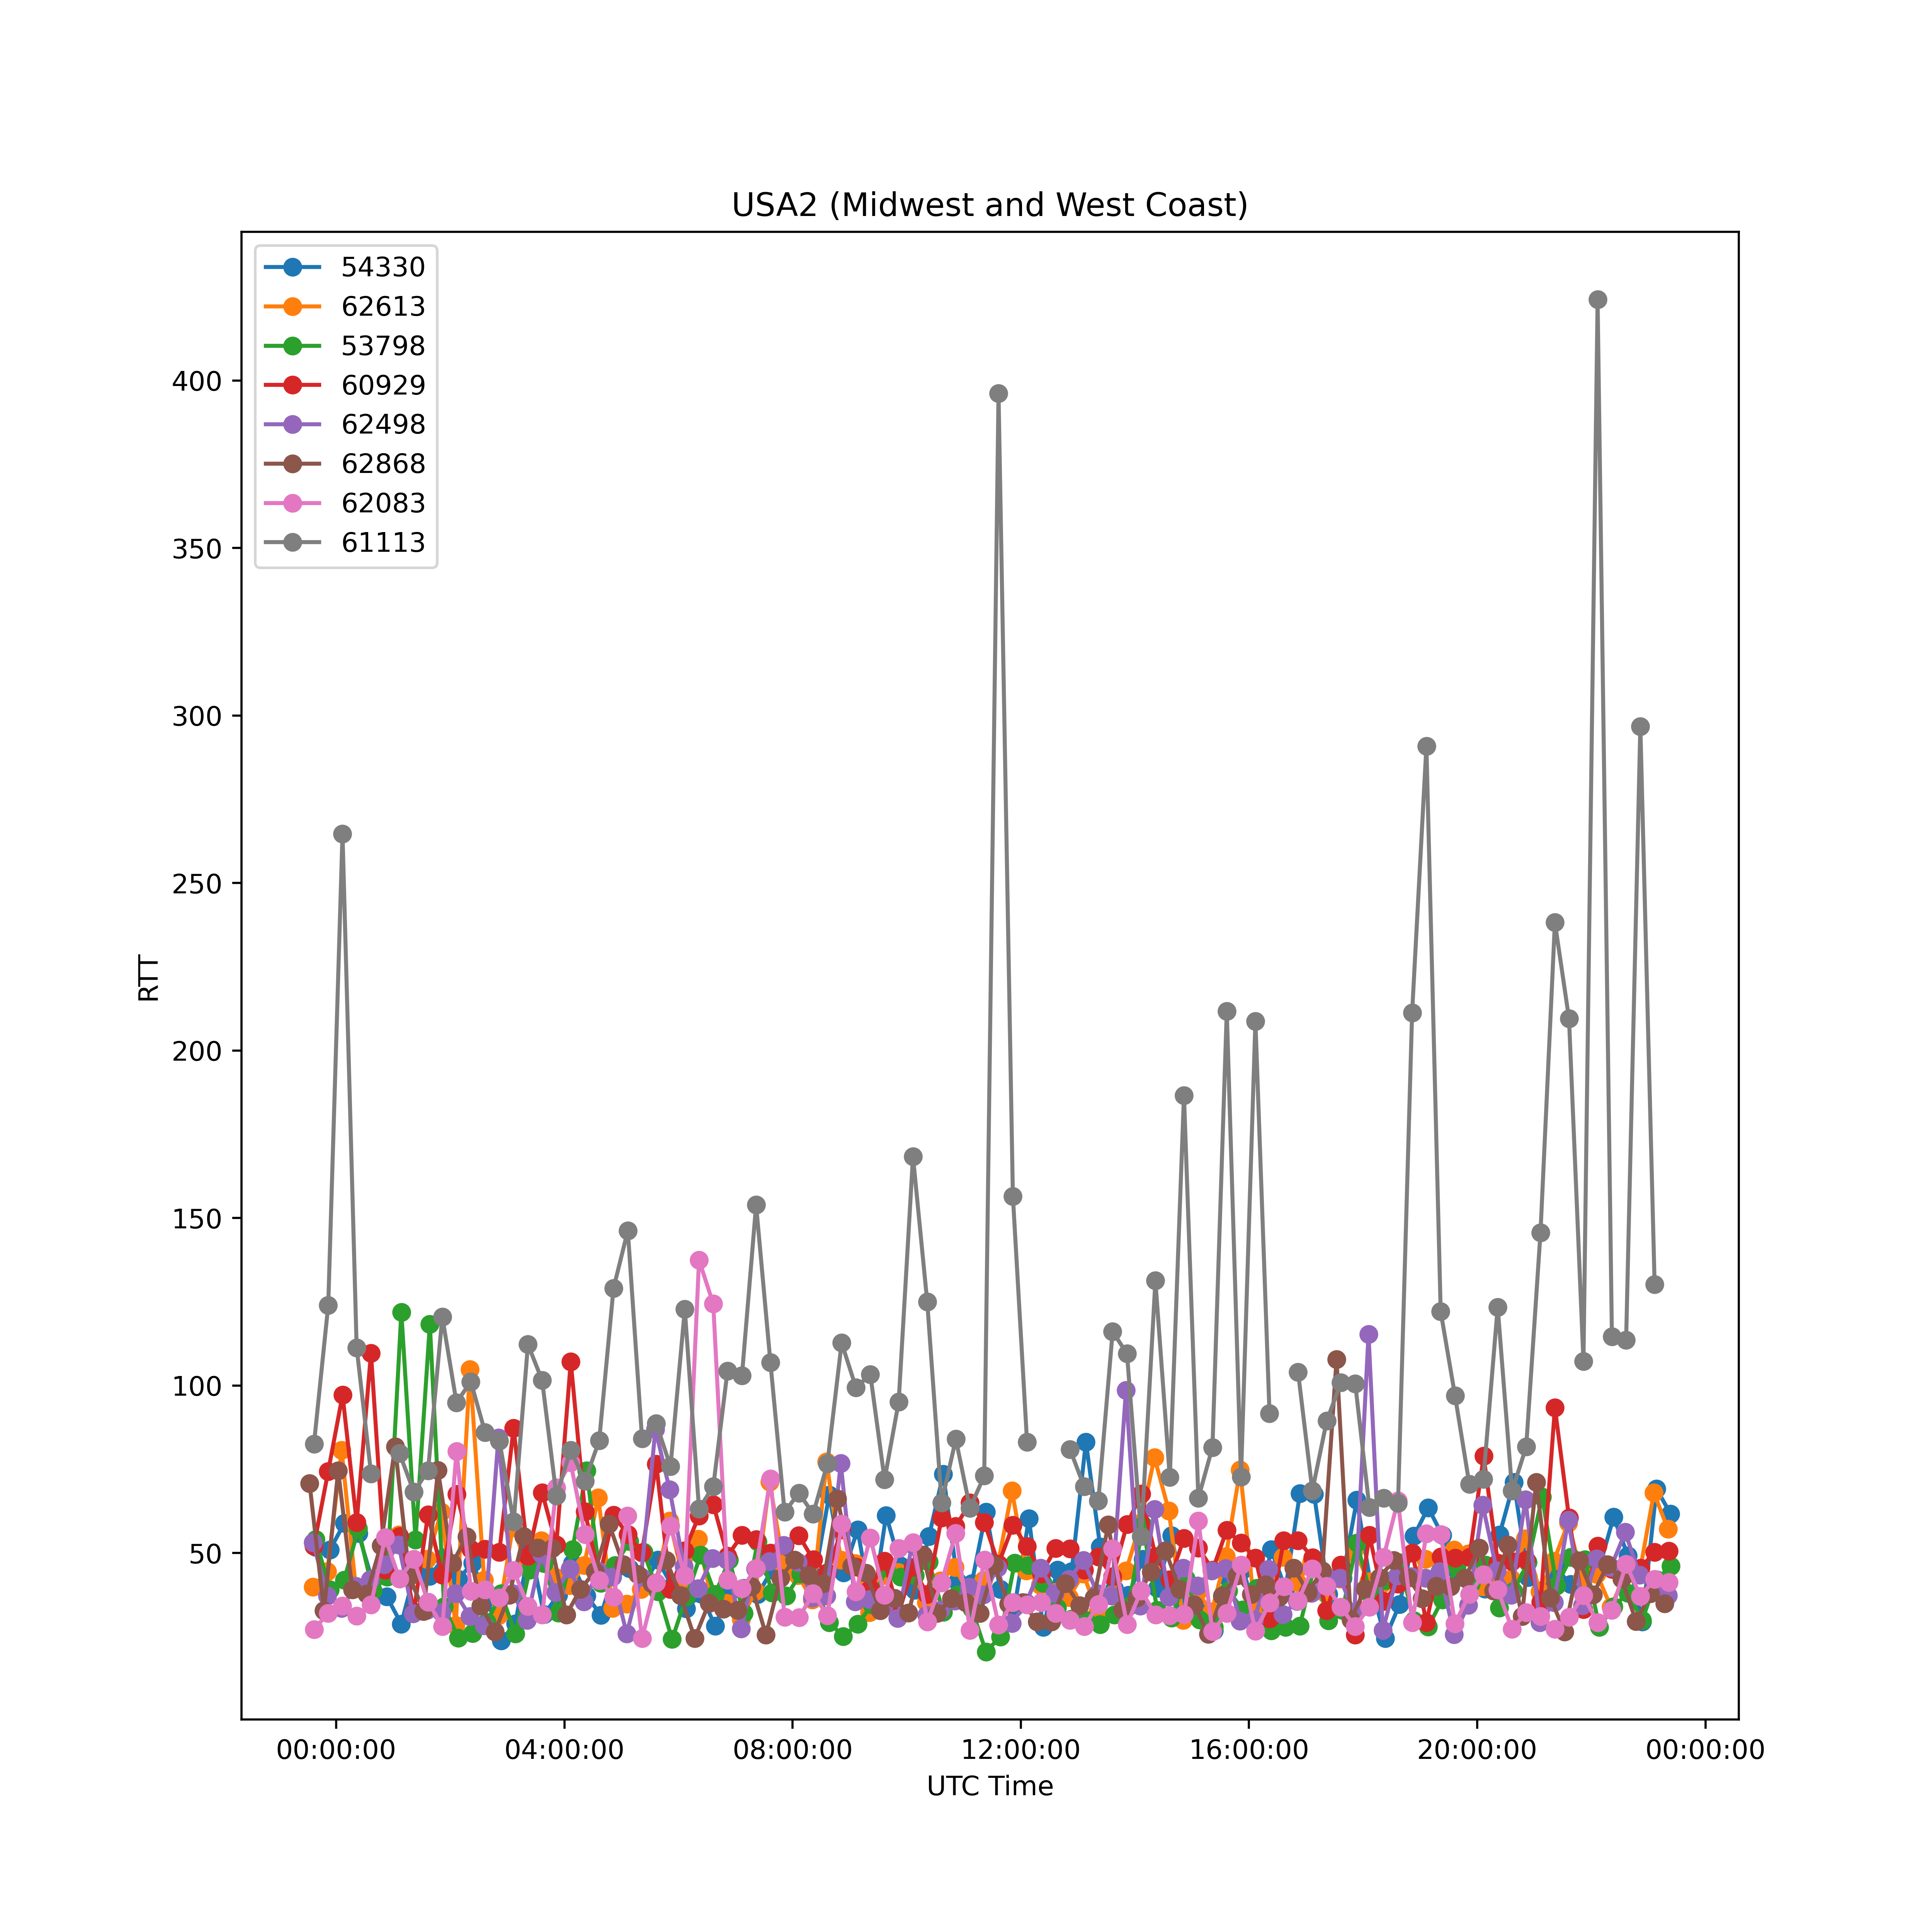
\includegraphics[scale=0.5]{graphs/usa2.png}
    \caption{Graph of RTT vs. UTC Time for the Midwest, West Coast, and Canada }
    \label{fig:usa2}
\end{figure}
    
TODO: describe east coast data

\subsubsection{Europe}
\begin{figure}
    \centering
    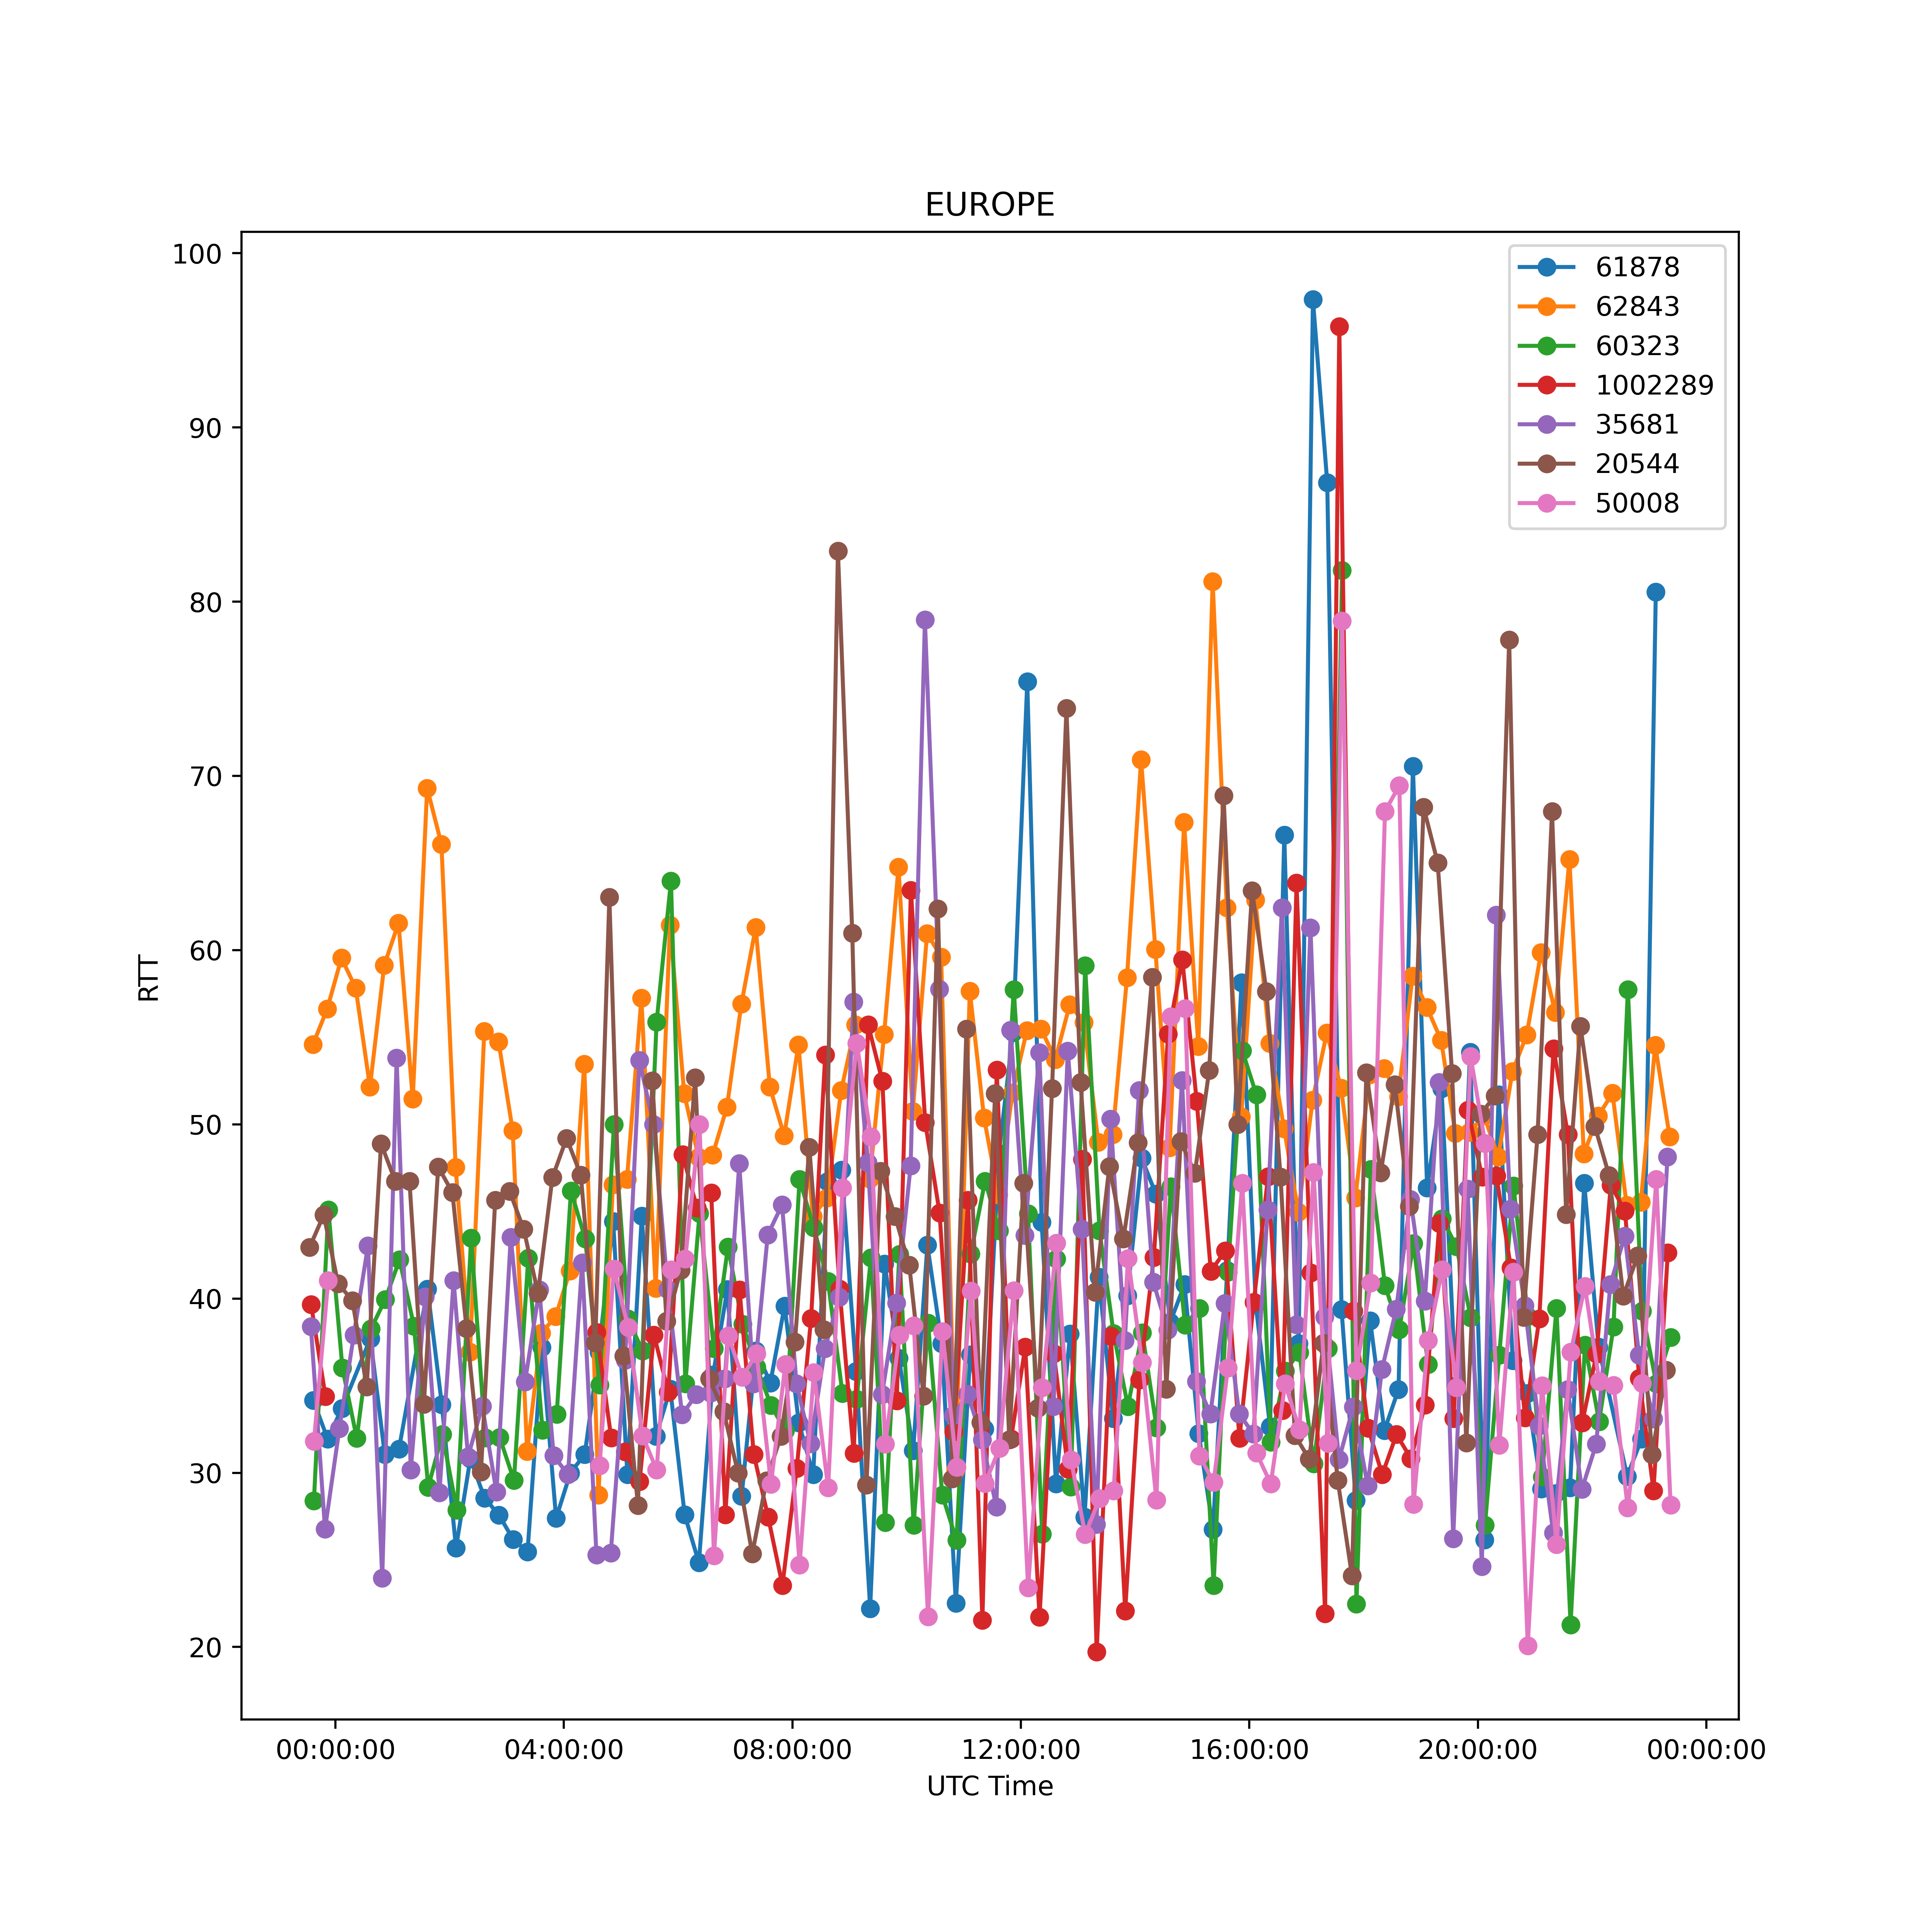
\includegraphics[scale=0.5]{graphs/eur.png}
    \caption{Graph of RTT vs. UTC Time for Europe}
    \label{fig:eruope}
\end{figure}
    
TODO: describe europe data

\subsubsection{Oceania}
\begin{figure}
    \centering
    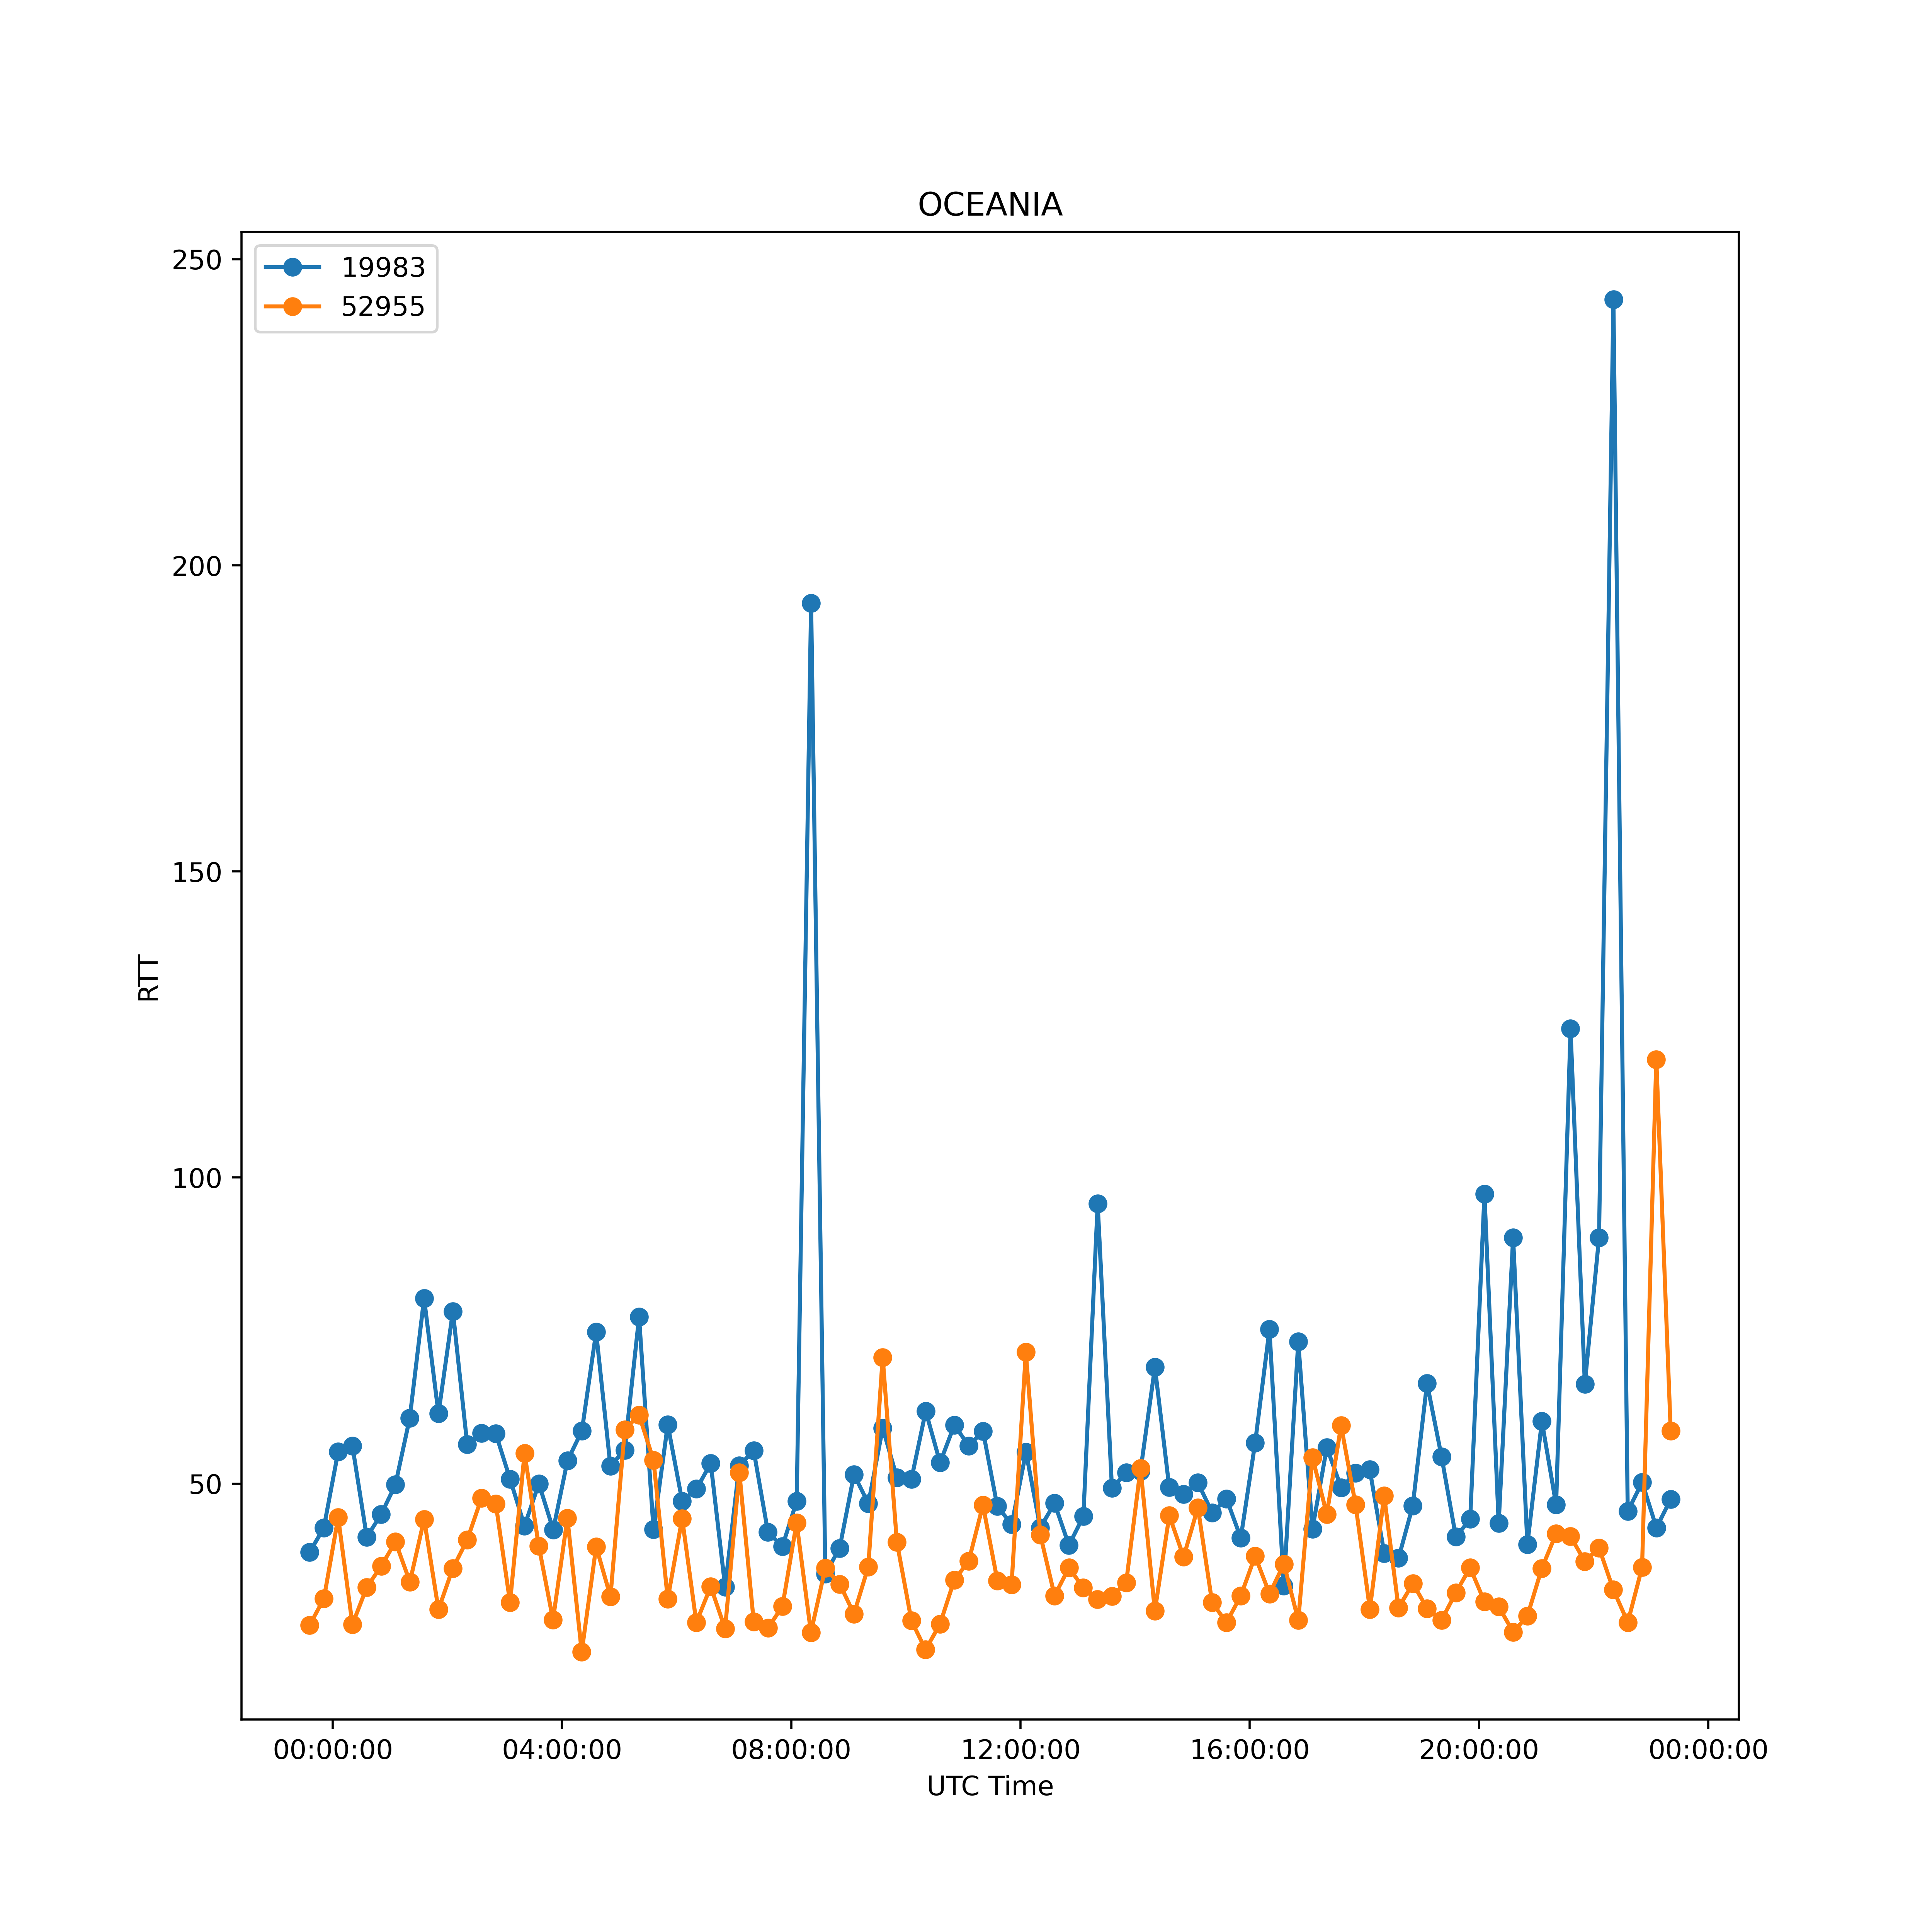
\includegraphics[scale=0.5]{graphs/oce.png}
    \caption{Graph of RTT vs. UTC Time for Oceania}
    \label{fig:oceania}
\end{figure}
    
TODO: describe oceania

\section{Analysis}

\subsection{USA1}

\subsection{USA2}

\subsection{Europe}

\subsection{Oceania}

\section{Conclusion}

\section{Selective Probing (Extra Credit)}



\section{Figures} 

% left this for reference

The ``\verb|figure|'' environment should be used for figures. One or
more images can be placed within a figure. If your figure contains
third-party material, you must clearly identify it as such, as shown
in the example below.
\begin{figure}[h]
  \centering
  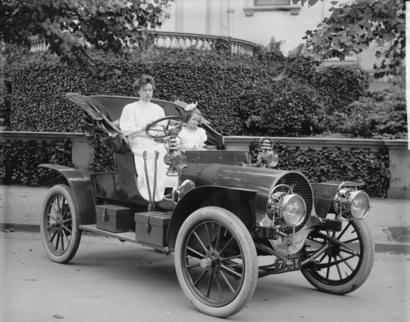
\includegraphics[width=\linewidth]{sample-franklin}
  \caption{1907 Franklin Model D roadster. Photograph by Harris \&
    Ewing, Inc. [Public domain], via Wikimedia
    Commons. (\url{https://goo.gl/VLCRBB}).}
  \Description{A woman and a girl in white dresses sit in an open car.}
\end{figure}

Your figures should contain a caption which describes the figure to
the reader.

Figure captions are placed {\itshape below} the figure.

Every figure should also have a figure description unless it is purely
decorative. These descriptions convey what’s in the image to someone
who cannot see it. They are also used by search engine crawlers for
indexing images, and when images cannot be loaded.

A figure description must be unformatted plain text less than 2000
characters long (including spaces).  {\bfseries Figure descriptions
  should not repeat the figure caption – their purpose is to capture
  important information that is not already provided in the caption or
  the main text of the paper.} For figures that convey important and
complex new information, a short text description may not be
adequate. More complex alternative descriptions can be placed in an
appendix and referenced in a short figure description. For example,
provide a data table capturing the information in a bar chart, or a
structured list representing a graph.  For additional information
regarding how best to write figure descriptions and why doing this is
so important, please see
\url{https://www.acm.org/publications/taps/describing-figures/}.

\subsection{The ``Teaser Figure''}

A ``teaser figure'' is an image, or set of images in one figure, that
are placed after all author and affiliation information, and before
the body of the article, spanning the page. If you wish to have such a
figure in your article, place the command immediately before the
\verb|\maketitle| command:
\begin{verbatim}
  \begin{teaserfigure}
    \includegraphics[width=\textwidth]{sampleteaser}
    \caption{figure caption}
    \Description{figure description}
  \end{teaserfigure}
\end{verbatim}

\section{Citations and Bibliographies}

The use of \BibTeX\ for the preparation and formatting of one's
references is strongly recommended. Authors' names should be complete
--- use full first names (``Donald E. Knuth'') not initials
(``D. E. Knuth'') --- and the salient identifying features of a
reference should be included: title, year, volume, number, pages,
article DOI, etc.

The bibliography is included in your source document with these two
commands, placed just before the \verb|\end{document}| command:
\begin{verbatim}
  \bibliographystyle{ACM-Reference-Format}
  \bibliography{bibfile}
\end{verbatim}
where ``\verb|bibfile|'' is the name, without the ``\verb|.bib|''
suffix, of the \BibTeX\ file.

Citations and references are numbered by default. A small number of
ACM publications have citations and references formatted in the
``author year'' style; for these exceptions, please include this
command in the {\bfseries preamble} (before the command
``\verb|\begin{document}|'') of your \LaTeX\ source:
\begin{verbatim}
  \citestyle{acmauthoryear}
\end{verbatim}

  Some examples.  A paginated journal article \cite{Abril07}, an
  enumerated journal article \cite{Cohen07}, a reference to an entire
  issue \cite{JCohen96}, a monograph (whole book) \cite{Kosiur01}, a
  monograph/whole book in a series (see 2a in spec. document)
  \cite{Harel79}, a divisible-book such as an anthology or compilation
  \cite{Editor00} followed by the same example, however we only output
  the series if the volume number is given \cite{Editor00a} (so
  Editor00a's series should NOT be present since it has no vol. no.),
  a chapter in a divisible book \cite{Spector90}, a chapter in a
  divisible book in a series \cite{Douglass98}, a multi-volume work as
  book \cite{Knuth97}, a couple of articles in a proceedings (of a
  conference, symposium, workshop for example) (paginated proceedings
  article) \cite{Andler79, Hagerup1993}, a proceedings article with
  all possible elements \cite{Smith10}, an example of an enumerated
  proceedings article \cite{VanGundy07}, an informally published work
  \cite{Harel78}, a couple of preprints \cite{Bornmann2019,
    AnzarootPBM14}, a doctoral dissertation \cite{Clarkson85}, a
  master's thesis: \cite{anisi03}, an online document / world wide web
  resource \cite{Thornburg01, Ablamowicz07, Poker06}, a video game
  (Case 1) \cite{Obama08} and (Case 2) \cite{Novak03} and \cite{Lee05}
  and (Case 3) a patent \cite{JoeScientist001}, work accepted for
  publication \cite{rous08}, 'YYYYb'-test for prolific author
  \cite{SaeediMEJ10} and \cite{SaeediJETC10}. Other cites might
  contain 'duplicate' DOI and URLs (some SIAM articles)
  \cite{Kirschmer:2010:AEI:1958016.1958018}. Boris / Barbara Beeton:
  multi-volume works as books \cite{MR781536} and \cite{MR781537}. A
  couple of citations with DOIs:
  \cite{2004:ITE:1009386.1010128,Kirschmer:2010:AEI:1958016.1958018}. Online
  citations: \cite{TUGInstmem, Thornburg01, CTANacmart}. Artifacts:
  \cite{R} and \cite{UMassCitations}.

\section{Acknowledgments}

Identification of funding sources and other support, and thanks to
individuals and groups that assisted in the research and the
preparation of the work should be included in an acknowledgment
section, which is placed just before the reference section in your
document.

This section has a special environment:
\begin{verbatim}
  \begin{acks}
  ...
  \end{acks}
\end{verbatim}
so that the information contained therein can be more easily collected
during the article metadata extraction phase, and to ensure
consistency in the spelling of the section heading.

Authors should not prepare this section as a numbered or unnumbered {\verb|\section|}; please use the ``{\verb|acks|}'' environment.

\section{Appendices}

If your work needs an appendix, add it before the
``\verb|\end{document}|'' command at the conclusion of your source
document.

Start the appendix with the ``\verb|appendix|'' command:
\begin{verbatim}
  \appendix
\end{verbatim}
and note that in the appendix, sections are lettered, not
numbered. This document has two appendices, demonstrating the section
and subsection identification method.



\end{document}
\endinput
%%
%% End of file `sample-acmsmall.tex'.
